


% \documentclass[a4paper]{article}
\documentclass[12pt,twoside,onecolumn]{article}
\usepackage{a4}
\usepackage{graphicx, fullpage, float, subfig, verbatim,amsmath, multirow, fancyhdr, hyperref}
\usepackage[utf8]{inputenc} 
\usepackage[norsk]{babel}
\usepackage{empheq}
\usepackage[dvipsnames,table]{xcolor}


%\title{\textbf{''Gisse GIS''  \\- webbasert geografisk informasjonssytem ved hjelp av Open Source-programvare}
%\\ \normalsize TBA 4251 - Programmering i geomatikk, høsten 2012}
%\author{Steffen Pøhner Henriksen}
%\date{\today}

\makeatletter
\def\thickhrulefill{\leavevmode \leaders \hrule height 1pt\hfill \kern \z@}
\def\maketitle{%
  \null
  \thispagestyle{empty}%
  \vskip 1cm
  \begin{flushright}
    \normalfont\huge\@title\par
  \end{flushright}
  \vfil
  \begin{flushright}
    \LARGE \strut \@author \par
  \end{flushright}
  \par
  \vfil
  \vfil
  \null
  }
\makeatother
\title{\textbf{''Gisse GIS''  \\- webbasert geografisk informasjonssytem ved hjelp av\\ Open Source-programvare}
\\ \normalsize TBA 4251 - Programmering i geomatikk, høsten 2012}
\author{Steffen Pøhner Henriksen}
\date{\today}
\begin{document}
\maketitle

\vspace{3cm}

\pagebreak

\begin{abstract}

	Gisse GIS er resultatet av min innsats i faget "TBA4251 - Programmering i geomatikk". Det er et enkelt geografisk informasjonssystem som kjører i en nettleser. Ved hjelp av Open Source-programvare vises vektordata over fritt tilgjenglige bakgrunnskart. Vektordataene kan så manipuleres med metoder kjent fra kraftfulle GIS som er desktop-applikasjoner. Metodene som støttes i dag er:
	
	\begin{itemize}
		\item Buffer - Utvider valgt område med en gitt verdi i meter.
		\item Area - Gir arealet av området i kvadratmeter.
		\item Merge - Slår sammen to vektorlag.
		\item Subtract - Trekker et vektorlag fra et annet.
		\item Intersect - Returnerer overlappende vektorlag.
		\item Distance - Finner minste avstand mellom to vektorlag.
		\item Simplify - Forenkler geometrien til et vektorlag ved Douglas-Peuker. 
	\end{itemize}
	
	Programmet består av tre deler - database, serverlag og klient. Kommunikasjonen mellom server og klient skjer via Websockets\cite{websockets}. Klienten er skrevet i Javascript, med HTML5 og CSS3. Tilleggsbiblioteker som er brukt i klienten er Knockout.js og jQuery, samt Twitter Bootstrap. Serverlaget er skrevet i node.js som tilbyr Javascript til bruk for serverkode. Her er sockets.io, Express og databasedriver brukt som tilleggsbiblioteker. Eksempeldata brukt i utviklingen og til demostrasjon er hentet fra Open Street Map og lagres i en PostgreSQL-database med PostGIS-utvidelse. Alt er lagret i skyen hos Amazons EC2-tjeneste, som sørger for at programmet leveres til brukers nettleser. 
	
	Resultatet er et brukervennlig GIS som utfører enkle operasjoner vi kjenner fra før, på frie vektordata som eksempel. ''Gisse GIS'' kan prøves ved å besøke adressen http://gisse.pohnerhenriksen.com i din nettleser.
	
\end{abstract}
\newpage

\tableofcontents
\newpage

\section{Innledning}
	
	Denne rapporten omhandler arbeidet med ''Gisse GIS'' utført høsten 2012. Den er et resultat av faget ''TBA4251 - Programmering i Geomatikk'' ved NTNU. Rapporten argumenterer for valg av programmeringsspråk, tilleggsbiblioteker og fremgangsmåte i arbeidsprosessen. Dataflyt og strukturen av programmet blir lagt frem. Et forslag til et scenario for å teste programmet blir også presentert. Oppdagede bugs, feil og mangler blir listet opp og kommentert. 
	
	Man kan dele inn arbeidet i fire deler - design, implementering, bugfiksing og rapportskriving. En stor del av arbeidet med utarbeidelsen av programmet var definere hva det skulle bli, hvilke verktøy som var hensiktsmessig å bruke, samt lære seg disse verktøyene. Tidlig ble det bestemt at jeg ville velge GIS-oppgaven i faget. Det gav meg muligheten til å jobbe med Javascript/HTML, noe jeg ikke har brukt i noen særlig grad før og har lyst til å lære meg. Oppgaven er farget av at jeg i størst mulig grad ville benytte meg av Open Source-programvare, og gjøre meg kjent med hva som finnes av slik programvare for bruk i geomatikkfaget. 
	
	\begin{quotation}
		"Software is like sex: it's better when it's free." 
			\em  -- Linus Torvalds
	\end{quotation}
	
	Tidligere har jeg jobbet hos Norkart AS som systemutvikler. Her laget jeg en database/server-løsning som behandlet geografiske data med tilleggsinformasjon. Kunnskapen fra denne sommerjobben kom godt med i utarbeidelsen av oppgaven. Kunnskapen opparbeidet herfra gjorde at jeg raskt så muligheter som PostGIS gir, og at implementeringen av databasedelen gikk relativt lett.
	
	\begin{figure}[h]
	\centering
	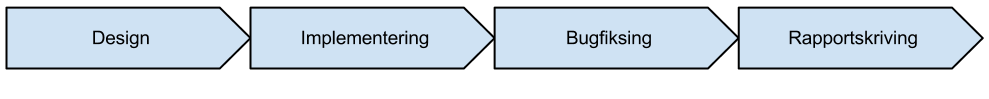
\includegraphics[scale=0.5]{innledning.png}
	\caption[Arbeidsprosess]{Arbeidsprosess}
	\end{figure}
	
\section{Formål med applikasjonen}

	Applikasjonen tilbyr brukeren et GIS med grunnleggende funksjoner som er tilgjenglig uavhengig av plattform. Den kjøres i alle moderne nettlesere. Det gjør ''Gisse GIS'' lett tilgjenglig, og enkelt å ta i bruk da det ikke krever noen installasjon utover å besøke en nettadresse. Funksjonene utføres raskt, og krever lite av klienten. Det er serveren som står for kalkulasjonene. Applikasjonen er ment som en inngansportal, og et demonstrasjonsverktøy for GIS. Man kan enkelt ved hjelp av åpne eksempeldata vise hvor kraftfullt et geografisk informasjonssytem kan være ved hjelp av enkle funksjoner. 
	
	Undertegnede håper også at kodegrunnlaget kan være et springbrett for andre studenter og GIS-interesserte til å lage nettbaserte kartløsninger. Kildekoden ligger fritt tilgjenglig på Github, og kan brukes fritt under OpenSource-lisensen. 
	
	I tillegg til funksjonene man kan utføre på vektordata er også mange ulike bakgrunnskart vist frem i applikasjonen. Disse kan brukes uavhengig av resten av programmet. Både kart, hybridkart og satelittbilder er tilgjenglig. Det finnes få eksempler på implementasjon av Kartverkets kart i websammenheng, og jeg håper koden kan hjelpe flere i å ta i bruk disse. Bedre kart finnes jo ikke over Norge! Og altfor få norske kartapplikasjoner tar i bruk Kartverkets kart. 

\section{Valg av programmeringsspråk og programbibliotek}
	
	Jeg var aldri i tvil om at det var GIS-oppgaven jeg ville velge. For å kunne nå ut til flest mulig brukere, uavhengig av maskinvarekonfigurasjon og plattform ville jeg bruke nettleseren. Da kunne også applikasjonen fungere på smarttelefoner og nettbrett i tillegg til desktop. Og dette uten å lage egne apps for disse.
	
	\subsection{HTML5 og CSS3}
		
		Med nettleseren som klient kommer man ikke unna HTML og CSS for å henholdsvis strukturere og designe en nettside. Jeg valgte å ta i bruk den nyeste standarden av HTML, HTML5. Dette gjorde det mulig å ta i bruk canvas-elementet for å tegne kart, og bruke rask nettverksoverføring via Websockets. Dette gjør at opplevelsen for brukeren med en moderne nettleser blir best mulig. HTML5 er også standarden i dag, og jeg fant det best å lære seg denne versjonen.
		
		CSS3 tilbyr en del nye funksjoner i forhold til den eldre CSS 2.0. Jeg har ikke tatt i bruk altfor mange av disse nye funksjonene, men gjort meg litt kjent med mulighetene. I applikasjonen har jeg rundet av hjørnene på menyene med kommandoer hentet fra CSS3. Dette skaper et mer helhetlig, rent og funksjonelt design. 
	
		\subsubsection{Twitter Bootstrap}
			
			Grunnet prosjektets tidsbegrensning og for enkelhetens skyld brukte jeg et rammeverk for å sette opp hjemmesiden. Dette heter Twitter Bootstrap, og gir muligheten til å bruke en hel del forhåndsdesignede elementer. Rammeverket er svært populært. Med dette kunne jeg lage navigeringsstripa på toppen, samt design på knapper. Hjelpesiden, og ''om meg'' involverer sterk bruk av dette rammeverket. Verktøymenyene er derimot laget spesielt for denne siden. Rammeverket er svært nyttig for såkalt "responsivt design". På den måten kan man lage nettsider som ser bra ut på store og små skjermer, også smarttelefoner og nettbrett. 
			
		\subsubsection{Leaflet}
		
			Kartet på siden tegnes av javascriptbiblioteket Leaflet. Dette er et nytt og moderne alternativ til det mer kjente Open Layers. Leaflet er kjent for å være bedre på små skjermer, samt enklere å bruke. Den tar i bruk canvas-elementet i HTML5. Jeg bruker Leaflet til å tegne GeoJSON-filer fra som mottas fra serveren, vise bakgrunnskart og popup-elementer. Den fungerer fint på nettbrett og smarttelefoner da klype-zoom støttes. Bakgrunnskart som er tilgjenglig er:
			
			\begin{itemize}
				\item Karverkets topografiske kart (farge og sort/hvitt)
				\item Karverkets topografiske rasterkart
				\item Cloudmade
				\item MapQuest
				\item OpenStreetMap
				\item Google (roadmap, satelitt og hybrid)
				\item To kreative kart
				\item Bing-satelittbilder
				\item MapQuest satelittbilder
			\end{itemize}
			
	\subsection{JavaScript}
	
		JavaScript brukes for å gi dynamisk innhold til nettsider, og er et naturlig valg i enhver webapplikasjon. Dette er et språk som bare blir mer og mer populært, og er spådd en stor fremtid. ''Gisse GIS'' tar i bruk javascript i mange deler av programmet. Og står for selve kjernen av koden. 
		
		\subsubsection{jQuery}
		
		jQuery er et støttebibliotek til javascript. Det finnes knapt javascript som ikke tar i bruk dette. Det forenkler kodeflyten, og kommandoene i javascript. Biblioteket legger flere og enklere verktøy i verktøykasse til webutvikleren. jQuery blandt annet for animasjonene av menyene, pekere på dynamisk innhold og menyhåndtering.
		
		\subsubsection{Knockout.js}
		
		Knockout.js implementerer Model-View-View-Model (MVVC) på en enkel måte i applikasjonen. Den holder styr på vektorlagene, og oppdaterer brukergrensesnittet om den oppdager noen endringer. På denne måten er det enkelt å holde applikasjonen konsistent, og alltid presentere brukeren de riktige dataene. Med Knockout.js kan jeg knytte metoder til hvert enkelt lag, og gjøre operasjoner som navneendring og fjerning lettere. Biblioteket holder regnskap over hvilke lag som blir valgt til å manipuleres. 
		
		\subsubsection{Node.js}
		
		Videre over på serverdelen gjør node.js at jeg kan skrive en webserver ved hjelp av javascript. Node kompilerer javascript-koden ned til C før den kjøres. Dette biblioteket er i vinden for tiden, og er en veldig spennende teknologi. Den praktiserer asynkron I/O-håndtering og er ''event-driven''. Det gjør at webserveren enkelt kan skalere og håndtere store brukermasser. I tillegg gjorde det serverkoden enkel å skrive da syntaksen er den samme som for klienten. Jeg har lenge ønsket å utforske mulighetene node.js tilbyr, og valgte derfor dette fremfor .NET eller Java-løsninger. Det har jeg ikke angret på.
		
		\subsubsection{Socket.io}
		
		Socket.io er en utvidelse av node.js. Det gjør det mulig for applikasjonen å ta i bruk websockets for raskere overføring av data. Dette er en ny standard i HTML5 som reduserer ''overhead'' og gjør at vektorlag sendes raskere mellom server og klient. Biblioteket støtter også tilbakefall på eldre teknologier som long-pulling for eldre nettlesere.
		
	\subsection{PostgreSQL - PostGIS}
		
		Dataene fra OpenStreetMap har blitt importert i en database som kjører på serveren. Jeg valgte PostGIS som databaseløsning, da denne er definitivt best på romlige spørringer. PostGIS ligger til grunn for de funksjonene som programmet tilbyr, og er kjernen i dette programmet. Alle funksjonene i programmet bygger bruker tilsvarende funksjoner i PostGIS. I den nyeste versjonen av PostGIS kan man spørre etter GeoJSON på vektorlag, og dette har forenklet visningen av dataene betraktelig. 
		

\section{Server i skyen - Amazon EC2}

	En av kriteriene i oppgaveteksten er ''Applikasjonen skal testast ut og gjerast tilgjengeleg for omverda. Er det ein Web-basert applikasjon må den installerast på eit område som ikkje vert sletta med studentbrukar''. For å oppnå dette leier jeg en server hos Amazon EC2. Denne kjører databasen, og serverdelen av programmet. I en begrenset periode er dette gratis. Om programmet ikke får en altfor stor brukermasse burde denne løsningen holde godt. Serveren overvåkes jevnlig, men det kan hende at en bruker kan fremtvinge en feil som fører til stopp. Om man opplever dette så send en mail til undertegnede. Serverdelen logger hvilke ip-addresser som bruker programmet, og hvilke vektorlag de etterspør.
	
	Jeg bruker også et eget domene, pohnerhenriksen.com, for å gjøre det enklere for brukere å koble seg til applikasjonen. Et subdomene ''gisse'' peker nå på Amazonserveren. Og addressen til programmet er da: http://gisse.pohnerhenriksen.com.  

\section{Testscenario}

	I dette kapittelet vil jeg skissere et testscenario som illustrerer hva ''Gisse GIS'' er kapabel til. Dette kan brukes som en veilledning, og vil kun vise enkelte av funksjonene applikasjonen tilbyr.
	\\ \\
	Vi bruker Trondheimsområdet som testområde. Først åpner vi applikasjonen ved å navigere til http://gisse.pohnerhenriksen.com i nettleseren. Programmet sentrerer seg i Trondheim ved oppstart og kontrollpanelet er synlig. Vi bytter til et kart med mer informasjon ved å trykke på ''Background map'' og velge Kartverkets topo2-kart. 
	
	Vi har en truet sjøfuglart i Jonsvatnet og Selbusjøen. Vi vil konstruere et verneområde rundt disse vannene, og finne ut hvilken del av dette området som ligger i Malvik kommune. Deretter vil vi finne avstanden til Trondheim sentrum og arealet av delen som verneområdet som ligger i Malvik.
	
	Vi begynner ved å trykke på knappen for å legge til et nytt lag. En dialogboks dukker opp og vi skriver Jonsvatnet og trykker på ''Add Layer'' for å legge til laget. Tilsvarende gjør vi for Selbusjøen. Vi husker på at det i dialogboksen står at dataene er sensitive til store og små bokstaver. For å zoome raskt til Jonsvatnet trykker vi på ''zoom'' i lagpanelet. For en enklere analyse slår vi sammen de to sjøene ved å velge merge-funksjonen, og lage et felles vannlag. Deretter huker vi av de to lagene slik at de slåes sammen. Det nye laget dukker opp i panelet. For å enklere se hva vi jobber med slår vi av alle lag bortsett fra det vi nettopp har lagt til ved å huke av huken i lagpanelet. Trykker nok en gang på zoom for å få et best mulig overblikk over dataene. Vi gir det nye laget et nytt navn for at det skal bli lettere å jobbe med. Det gjør vi ved å trykke på ''edit'' og skrive inn ''Vann''.  For å lage et verneområde ønsker vi en utvidelse av lagene med 2km. Det gjør vi ved å velge buffer-funksjonen. Vi velger laget vi ønsker buffer på, og skriver 2000 i dialogboksen før vi trykker på ''Add buffer''. Et nytt lag blir lagt til i panelet. Nå kan vi endre navnet på dette laget til ''Verneområde''. Nå vil vi vite hvilken del som av dette verneområdet som ligger i Malvik kommune. Vi trykker på ''Add new layer'' for å legge til Malvik. For å kunne lage et lag av overlappen mellom Malvik og verneområdet bruker vi intersect-funksjonen. Vi velger Malvik og verneområdet og finner overlappen. For å se bedre på hvor dette området er bytter vi til et satelittbilde via ''Background map''-knappen, og skrur av alle lag bortsett fra det siste vi la til. Arealet fåes ved å å bruke area-funksjonen og velge laget. En liten dialogboks viser arealet i kvadratmeter i noen sekunder.	For å finne avstanden mellom Trondheim sentrum og området legger vi til et lag som er Marinen. Og bruker deretter Distance-funksjonen. Vi velger Marinen og overlapplaget og minste avstand dukker opp. For å vise frem området i kommuneplanen vil vi ha en forenklet utgave. Simplify kan hjelpe oss med det. Vi velger Simplify og laget vårt, og får tilbake en forenklet utgave. Vi endrer navnet til "Verneområde sjøfugl". Dermed har vi konstruert verneområdet. 
	

\section{Bugs, feil og mangler}

	Programmet er i jevnlig utvikling, og jeg vil fortsette å utvikle det etter dette prosjektet har blitt vurdert. Slik det fremstår i dag (25.12.2012) inneholder programmet en rekke feil eller bugs. Noen er mer kritiske enn andre. Applikasjonen har blitt testet på andre personer enn undertegnede. Både studenter i Geomatikk og andre personer bruker programmet på en måte jeg ikke så for meg. Og i denne bruken har det dukket opp flere feil. Noen av disse er:
	
	\begin{enumerate}
		\item Kontrollmenyen ligger feil på nettbrett
		\item Case-sensitive navn på eksempeldata forvirrer
		\item Lange navn på lag flytter på knappene
		\item Ved endring av navn (''Edit-knapp'') flytter ofte navigasjonsstripa på seg.
		\item Ved besøk av hjelpeside eller ''om meg'' lagres ikke arbeidet.
		\item Enkelte eksempeldata som ''Nidelva'' vil ikke utføres funksjoner på.
		
	\end{enumerate}
	
	
	\subsection{Forbedringspotensiale}
	
	Programmet kjører ikke på smarttelefoner, og ikke optimalt på nettbrett. Her finnes et stort forbedringspotensiale. Det krever en hel del arbeid for å få dette til å fungere. Med mindre skjermareal må menyer skjules på en annen måte enn de gjøres i applikasjonen i dag.
	
	Designet har også et forbedringspotensiale. I dag mynter programmet veldig på ''Twitter Bootstrap'', og det er ønskelig å lage et mer spesielt og annerledes design. Her kreves det tid i CSS-koden. I utviklingen av programmet har tidsbegrensningen tvunget meg til å fokusere på funksjonalitet.
	
	En bedre hjelpetjeneste kunne vært laget for å veillede nye brukere. Med dette kunne også programmet lyktes bedre i undervisningssammenheng. En interaktiv tutorial hadde vært morsomt å få til, men lå utenfor denne oppgaven. 
	
\section{Diskusjon - Løser applikasjonen oppgaven?}
	Slik jeg tolker oppgaven er den å lage et GIS med enkel funksjonalitet, som er bra ut og er enkelt å bruke. Den skal fungere på et utvalgt sett med eksempeldata. Jeg mener at ''Gisse GIS'' oppfyller disse kriteriene. Programmet kunne ha vært enda enklere å bruke, spesielt for de som ikke kjenner til geografiske informasjonssytem fra før av. Design er subjektivt, men jeg mener at programmet virker attraktivt samtidig som det er lett å finne funksjonene. Programmet er vektorbasert noe som betyr at det stilles andre krav enn ved rasterbaserte applikasjoner.
	
	Funksjonene som utføres på vektordataene har jeg ikke kodet selv. Dette står PostGIS for. Slik jeg ser det sier oppgaven ingenting om at det ikke er lov å bruke tilleggsbiblioteker av denne typen. Og det er nettopp ved hjelp av disse applikasjonen fremstår som lett å bruke og attraktiv, samtidig som den inneholder robust og viktig GIS-funksjonalitet. Ved å ha tatt i bruk av dette har jeg lært hvilke verktøy som er aktuelle i GIS-verdenen på web i dag, og har kunnet kunnet lage en funksjonsrik applikasjon på så kort tid.

\section{Problemer underveis}

	Utviklingen av en ny applikasjon er alltid heftet med problemer. Og utviklingen av ''Gisse GIS'' er intet unntak. JavaScript hadde jeg liten erfaring med fra før og skapte litt hodebry. 
	
	Node.js støtter seg på filosofien om asynkron I/O, og bruker derfor ofte såkalte ''callback''-funksjoner. Dette var en ny tankegang å følge for undertegnede. Men etter å ha lest en del artikler og sett en del eksempelvideoer ble utfordringene løst.
	
	Det var også problemer med at popupdialogene til Twitter Bootstrap ikke fanget museklikk, men de ble heller tatt imot av kartet. Det samme gjaldt tastatur. Til slutt besluttet jeg å gå bortifra disse popupdialogene kalt ''modals'', og heller lage noe eget. Dette fungerte etterhvert slik det var tiltenkt.
	
	Som nevnt tidligere i rapporten kjører ikke ''Gisse GIS'' godt på smartelefoner og nettbrett. Det ble gjort forsøk på å forbedre dette, men uten stort hell. Dette er et vanskelig problem som krever en del kunnskap, som jeg ikke har på nåværende tidspunkt.
	
	Det var også en del problemer med overføring av database/server fra en lokal produksjonsserver på min egen PC til skyen. Her krevdes det kjennskap til UNIX-kommandoer og kommandolinjen. Men dette ble løst etter nok knoting.    
	

\newpage
\begin{thebibliography}{9}

\bibitem{websockets}
	Wikipedia: Websockets, http://en.wikipedia.org/wiki/WebSocket, 22.12.2012

\end{thebibliography}

\listoffigures

\end{document}

